\section{Η προσέγγισή μας}\label{our_approach}

Η προσέγγισή μας έχει 3 βασικά μέρη:
\begin{itemize}
	\item \textbf{Κατάτμηση} των PCG δειγμάτων στις βασικές περιοχές του καρδιακού
	      ήχου.
	\item \textbf{MFCC μετασχηματισμό} των PCG δειγμάτων σε αναπαράσταση
	      χρόνου-συχνότητας της κατανομής της ενέργειας του σήματος.
	\item \textbf{Εκπαίδευση \& Κατηγοροποίηση} των MFCC heat maps με την χρήση
	      του συνελικτικού νευρωνικού δικτύου.
\end{itemize}

\subsection{Κατάτμηση Δειγμάτων}

Για να κάνουμε την κατάτμηση των PCG δειγμάτων όπως φαίνεται στην εικόνα
\ref{PCG} θα χρησιμοποιήσουμε των αλγόριθμο του Springer
\cite{springer2015logistic} τον οποίο τον παρείχε ο διαγωνισμός στους
συμμετέχοντες. Ωστόσο δεν θα χρησιμοποιήσουμε όλα τα δεδομένα που μας δίνει ο
αλγόριθμος, αλλά αυτό που θα κάνουμε είναι να βρίσκουμε που ξεκινάει το πρώτο
\emph{S1} και στη συνέχεια θα αναλύουμε τα 3 επόμενα δευτερόλεπτα. Αυτή η
διαδικασία θα γίνεται ώστε τα δείγματα με τα οποία θα εκπαιδεύσουμε το νευρονικό
δίκτυο να είναι ``ευθυγραμισμένα'' μεταξύ τους.


\subsection{Μετασχησματισμός MFCC}

Αφού πάρουμε τα 3 δευτερόλεπτα σκοπός είναι να δημιουργήσουμε μια εικόνα που θα
\textbf{κουβαλάει} χαρακτηριστικά του ηχητικού αποσπάσματος ώστε να μπορέσουμε 
να προπονήσουμε το νευρονικό μας δίκτυο. Αυτό μπορούμε να το πετύχουμε υπολογίζοντας
τις MFCC τιμές του καρδιγραφήματος με την εξής διαδικασία:
\begin{enumerate}
  \item Παίρνουμε επικαλυπτόμενα παράθυρα πάνω στο ηχητικό δείγμα
  \item Υπολογίζουμε τον μετασχηματισμό Fourier για κάθε παράθυρο
  \item Εφαρμόζουμε τα Mel φίλτρα και αθροίζουμε τις ενέργιες σε κάθε φίλτρο
  \item Υπολογίζουμε τις λογαριθμικές τιμές των παραπάνω ενεργειών
  \item Τέλος παίρνουμε τον διακριτό συνημιτονικό μετασχηματισμό των λογαριθμικών
    τιμών.
\end{enumerate}

Έτσι θα έχουμε 12 MFCC τιμές για κάθε παράθυρο και μαζί με το ολική ενέργεια
του παραθύρου ως ξεχοριστή τιμή παίρνουμε 13 τιμές. Αναπαριστώντας αυτά
χαρακτηριστικά σε ένα γράφημα όπου ο $y$ άξονας θα κυμαίνετε από 0 εώς 12 (μία
γραμμή για κάθε MFCC τιμή) και ο $x$ άξονας από 0 εώς $3000 / step\_size$
(\emph{step\_size} που θα ορίσουμε για κάθε παράθυρο), θα πάρουμε ένα heat map
(βλέπε \ref{mfcc}) που μπορούμε να χρησιμοποιήσουμε ως εικόνα για το νευρονικό
δίκτυο.

\begin{figure}[H]
  \center
	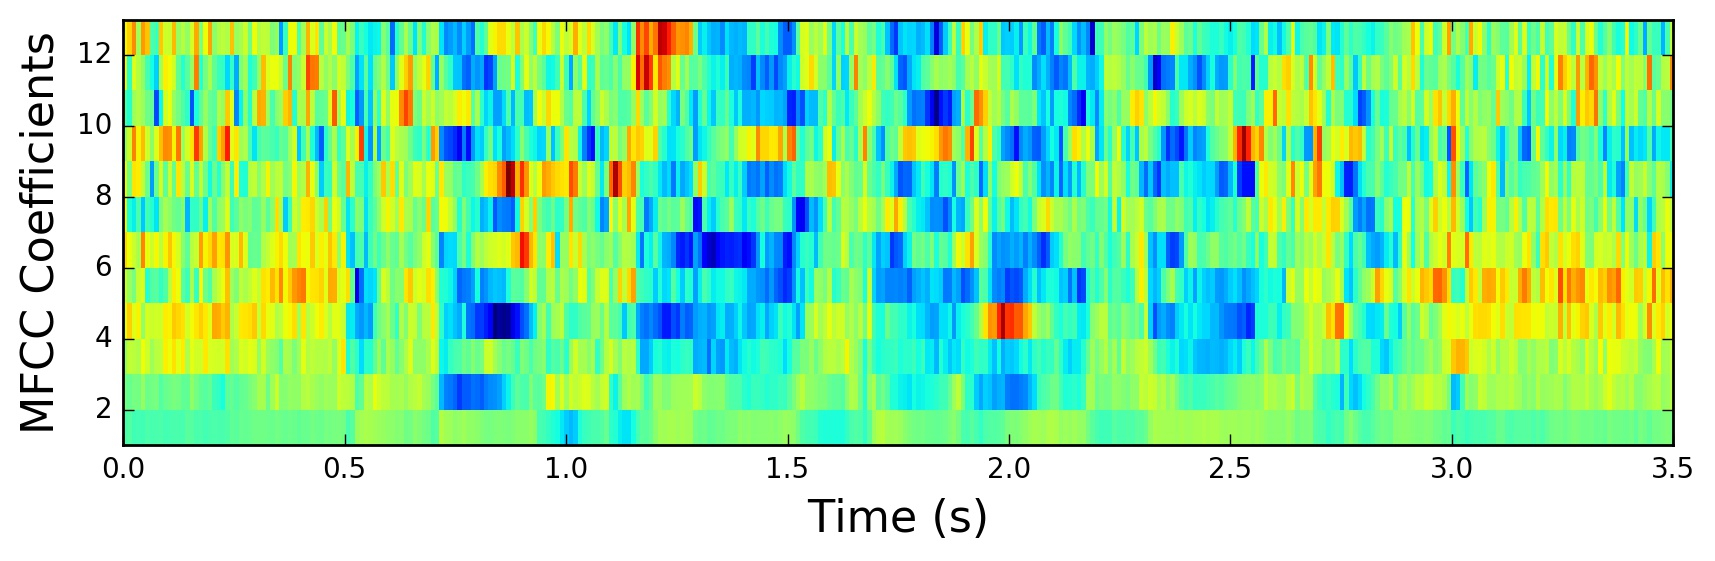
\includegraphics[width=0.5\textwidth]{mfcc.jpeg}
  \caption{MFCC heat map \cite{fayek2016}}
	\label{mfcc}
\end{figure}

\subsection{Νευρωνικό δίκτυο}
\subsubsection{Αρχιτεκτονική δικτύου}
